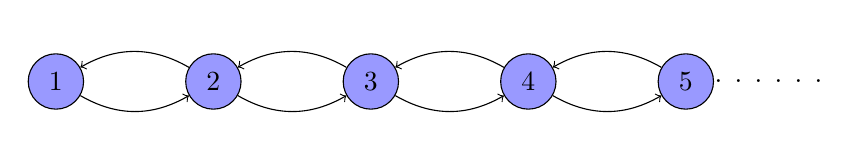
\begin{tikzpicture}
\tikzstyle{every node}=[draw,circle,fill=blue!40!white,minimum size=20pt,
inner sep=0pt]

\draw (3,0)  node (2)  {2};
\draw (5 ,0)  node (3)  {3};
\draw (1,0)  node (1)  {1};
\draw (7,0)  node (4)  {4};
\draw (9,0)  node (5) [label=right:  . . . . . .]  {5};
\draw [->] (2) to  [bend right] (1);
\draw [->] (2) to  [bend right] (3);
\draw [->] (1)to  [bend right](2);
\draw [->] (3)to  [bend right](2);
\draw [->] (3) to  [bend right] (4);
\draw [->] (4) to  [bend right] (3);
\draw [->] (4) to  [bend right] (5);
\draw [->] (5) to  [bend right] (4);

\end{tikzpicture}